\chapter{Related Work}


\section{SPARQL approach}
DEANNA [28] allows users to input questions in natural language and generates queries over a knowledge base that return answers. It then translates these questions into a structured SPARQL query that can be evaluated over knowledge bases such as Yago, Dbpedia, Freebase, or other Linked Data sources. 

\section{Querying by example entity tuples}
 GQBE [29] proposes to query knowledge graphs by example entity tuples, where the users do not have to construct any query graph. 
 
 GQBE is a system that queries entity-relationship graph by example entity tuples. GQBE automatically creates a maximal query graph based on the input example query tuple and finds the top-K matching answer tuples. GBQE uses the notion of neighborhood graph and maximal query graph.
 
Given an entity-relationship graph G and a query tuple t, the corresponding
neighborhood graph H\textsubscript{t} is the weekly connected sub graph of G that consists of all undirected paths in G of length d or smaller, with at least one end point each such path being a query entity in t. The path length threshold d is an input parameter.

Even after removal of unimportant edges the reduced neighborhood graph Ht
 can be
quite large even under a small path length threshold d. The query evaluation cost can be very
high in finding approximate answers to such a large H\textsubscript{t}
. Hence we aim to drastically reduce the
size of H\textsubscript{t}
 and obtain a small subgraph that capture only important features of the input entities.
This graph is termed as maximal query graph G\textsubscript{t}
.
To obtain maximal query graph, edges in the reduced neighborhood graph weighted by
following measures.
Participation degree p(e) of an edge e =(u, v) define as number of edges
in data graph which share the same edge label and at least one of the two end nodes of edge e.

For edge e, Inverse Edge Label Frequency is defined as,

\begin{align}
ief(e) = \frac{ log | E(G) | }{ \#label(e)}
\end{align}


Where $|$E(G)$|$ is the number of edges in data graph G and \#label(e) is the number of edges in G with the same label as e.

So, given a input query tuple t, its reduced neighborhood graph H\textsubscript{t}
, and a parameter m, the
maximal query graph Gt
 is a weekly connected subgraph of Ht
 that maximize total edge weight
and it has m edges. Here weight of edge e define as,

\begin{align}
w(e) = \frac{ief (e)}{p(e) \times d^2(e)}
\end{align}


Here d(e) is smallest distance of edge e from any input entity. 

 
\section{Interactive queries using user input}
 FreeQ [32] offers an interactive query interface over Freebase that enables a naive user to start with simple keywords and incrementally refine them into a structured query that can accurately express the user’s informational need. \\
 
The conceptual process of incremental query construction can be modeled as follows:
\begin{itemize}
\item 
Given a database whose schema is G = (V,E), a user
issues a keyword query K = {k1, k2, ..., kn}. 
\item The system generates all possible query interpretations of K based on G. We call this set of query interpretations the interpretation space of K, denoted by ζ. 
\item The system generates an interaction option IO and presents it to the user. 
\item If the user accepts IO, then the system removes all the query interpretations that cannot imply IO from ζ. Otherwise, the system removes all the interpretations that imply IO from ζ.
\item The system retrieves the top-k query interpretations
from ζ, and presents them to the user. 
\item If the user finds the intended query interpretation from the top-k, the query construction process terminates. Otherwise, the process generates another interaction option IO and
presents it to the user.
\end{itemize} 

\section{Query interpretation based on history}
Fu and Anyanwu [33] propose a context-aware approach for keyword query interpretation that personalizes the interpretation process based on a user’s query context.

In this paper, the problem of generating context-aware query interpretations
for keyword queries on RDF databases by using information from
a user’s query history is addressed. The rationale for this is that users often pose a series of
related queries, particularly in exploratory scenarios. In these scenarios, information
about previous queries can be used to influence the interpretation of a
newer query. For example, given a keyword query “Mississippi River”, if a user
had previously queried about “Mortgage Rates”,then it is more reasonable to
select the interpretation of the current query as being that of a financial institution
“Mississippi River Bank”. On the other hand, if a user’s previous query was
“Fishing Techniques”, it may make more sense to interpret the current query
as referring to a large body of water : the “Mississippi River”. Two main challenges
that arise here include (i) effectively capturing and efficiently representing
query history and (ii) effectively and efficiently exploiting query history during
query interpretation.

The paper proposes and implements a dynamic weighted summary graph model that is
used to concisely capture essential characteristics of a user’s query history.

To achieve this effect, we designed the dynamic weighting function to be
based on a relevance function in terms of two factors: historical impact factor
(hif) and region factor (rf).
Let T indicate the historical index of the most recent query QT , t be the
historical index of an older keyword query Qt, i.e., t $<$ T, and m denote a
summary graph element. Assume that the top-1 interpretation for Qt has already
been generated : QI\textsubscript{t}. Region factor is defined as a monotonically decreasing
function of the graph distance d(m, QIt) between m and QIt:
\begin{align}
rf(d(m, QI\textsubscript{t})) = \frac{1} {a^{d(m,QI\textsubscript{t})}}
\end{align}
Here, a $>$ 1 is a positive integer constant.

Historical impact factor captures the
property that the relevance between a query and a graph element will decrease
when that query ages out of the query history. hif is a monotonically decreasing
function: 
\begin{align}
hif(t) = \frac{1}{b^{T-t}}
\end{align}
where b $>$ 1 is also a positive integer constant.


\section{Alternate query languages}
Pound et al. [30] approach the keyword disambiguation problem by ranking different possible rewritings of a query based on their syntactic relationship to the keywords in the query as well as their semantic coherence in the underlying knowledge base. 

In case of unstructured data,
data can be of any type, not necessarily follow any format or rule. e.g. text,video,sound etc. On the other
hand, in case of structured data, the data is organized in semantic chunks(entities). Similar entities are
grouped together to form relations or classes. i.e. in case of structured data, some schema information is
available. As an example ExDB,YAGO have schema items numbering in the millions. So, given such huge
schema information, writing a structured query is a very hard task. This is called Information Overload
Problem. As a naive approach to the above problem, one can use keyword search. But, this comes at a loss of expressivity.
i.e. users can not express desired structure in the query and can not take advantage of schema
information. But, it is very flexible, in the sense that a user can query even if he has no knowledge of the
underlying schema information. On the other hand, conventional structured query is expressive but lacks
flexibility. So, the authors propose a new approach that combines flexibility of keywords as well as expressivity
of structured query, to provide a new query language, called keyword-based structured query
language. e.g. say the information need is “find all people of German nationality who have won a Nobel
award”. Then, the structured query would be
“q(x):- GERMAN PEOPLE(x), hasWonPrize(x, y), NOBEL PRIZE(y)”. The keyword query would be “german
has won nobel award”, and the keyword basedstructured
query would be “german, has won(nobel award)”.


A user enters keyword-based structured query Q to the system. Each keyword k in Q is matched to a set
of schema items using some syntactic similarity measure, with the help of the KB. Each such set forms a
partition. Now, a disambiguation graph G is generated from these. Any induced subgraph of G, that spans
all the partitions, corresponds to a concept query interpretation of Q. Now, these interpretations are ranked
based on some score function that combines semantic and syntactic similarities with the original query Q,
given the KB. Next, top k of those structured queries are evaluated to find potentially relevant entities
and their corresponding documents. The documents are then returned to the user ranked by some relevance
metric.

MashQL [31] present a query formulation language in order to easily query and fuse structured 
data on the web where users can specify filters. It is designed without loss of generality and 
can be used for querying relational databases, XML, RDF and web tables. 

\section{Corpus}
35 propose two new, natural formulations for joint query interpretation and response ranking that exploit bidirectional flow of information between the knowledge base and the corpus.

Here  we  focus  on  a  specific  kind  of  entity  search  query:
Some words (called
selectors
) in the query are meant to occur literally in a response document (as in traditional text
search),  but other words
hint at the type of entity sought
by the query.  Unlike prior work on translating well-formed
sentences or questions to structured queries using deep NLP,
we are interested in handling "telegraphic" queries that are typically sent to search engines.  Each response entity must
be a member of the hinted type.
Note that this problem is quite different from finding answers  to  well-formed  natural  language questions (e.g., in
Wolfram Alpha) from structured knowledge bases (perhaps
curated through information extraction). Also observe that
we do not restrict ourselves to queries that seek entities by
attribute  values  or  attributes  of  a  given  entity  (both  are
valuable query templates for e-commerce and have been re-
searched).   In  our  setup,  some  responses  may  only  be  collected from diverse, open-domain, free-format text sources.
E.g., typical driving
time
between Paris and Nice (the target
type is time duration), or
cricketers
who scored centuries at
Lords (the target type is cricketers).
The  target  type  (or  a  more  general  supertype,  such  as
sportsperson
in place of
cricketer
) may be instantiated in a
catalog
, but the typical user has no knowledge of the catalog
or  its  schema.   Large  catalogs  like  Wikipedia or Freebase
evolve "organically".  They are not designed by linguists, and
they are not minimal or canonical in any sense.  Types have
overlaps  and  redundancies.   The  query  interpreter  should
take advantage of specialized types whenever available, but
otherwise gracefully back o to broader types.


----------------------------
36
We  present  a  new  architecture  for  structural  interpretation of a telegraphic query into these segments:
•
Mention/s
\^{e\textsubscript{1}}
of an entity
e\textsubscript{1}
,
•
Mention
\^{r}
of a relation type
r
,
•
Mention
\^{t\textsubscript{2}}
of a target type
t\textsubscript{2}
, and
•
Other  contextual  matching  words
s
(some-
times called
selectors
),
with the intent of finding and ranking entities
e\textsubscript{2} $ \in $
t\textsubscript{2}
,  such that
r
(e\textsubscript{1}
, e\textsubscript{2})
is likely
to hold.
Given  the  short,  telegraphic  query  utterances,
we limit our scope to at most one relation mention,
unlike  the  complex  mapping  of  clauses  in  well-
formed  questions  to  twig  and  join  style  queries
(e.g., “find an actor whose spouse was an Italian
bookwriter”). We  present  a  novel  discriminative  graphical
model to capture the entity ranking inference task.

The following notations are used:
\begin{itemize}


\item
$ \Psi $\textsubscript{R}
(q,z,r)
denotes   the   compatibility   be-
tween  the  relation  hint  segment
\^{r} (q,z)
and
a proposed relation type
r
in the KG.
\item 
$ \Psi $\textsubscript{T\textsubscript{2}}
(
q,z,t\textsubscript{2}
)
denotes  the  compatibility  between  the  type  hint  segment
\^{t\textsubscript{2}}
(
q,z
)
and  a
proposed  target  entity  type
t\textsubscript{2}
in  the KG.
\item
$ \Psi $\textsubscript{
E\textsubscript{1}
,R,E\textsubscript{2}
,S}
(
q,z,e\textsubscript{1}
,r,e\textsubscript{2}
)
is a novel corpus-
based evidence potential that measures how
strongly
e\textsubscript{1}
and
e\textsubscript{2}
appear in corpus snippets
in the proximity of words in
\^{s}
(
q,z
)
, and apparently related by relation type
r.
\item
$ \Psi $\textsubscript{
E\textsubscript{1}}
(
q,z,e\textsubscript{1}
)
denotes  the  compatibility  be-
tween the query segment

\^{e\textsubscript{1}}
(
q,z
)
and entity
e\textsubscript{1}
that it purportedly mentions.
\item
$ \Psi $\textsubscript{
S}
(
q,z
)
denotes selector compatibility.  Selectors are a fallback label, so this is pinned
arbitrarily to 1; other potentials are balanced
against this base value.
\item
$ \Psi $
\textsubscript{E\textsubscript{1}
,R,E\textsubscript{2}}
(
e\textsubscript{1}
,r,e\textsubscript{2}
)
is
A
if   the   relation
r
(
e\textsubscript{1}
,e\textsubscript{2}
)
exists in the KG, and is
B $>$
0
otherwise, for tuned/learnt constants
A $>$ B $>$ 0
. Note that this is a soft constraint (
B $>$
0
);
if the KG is incomplete, the corpus may be
able to supplement the required information.
\item
$ \Psi $\textsubscript{
E\textsubscript{2}
,T\textsubscript{2}}
(
e\textsubscript{2}
,t\textsubscript{2}
)
is  1  if
e\textsubscript{2}
belongs  to
t\textsubscript{2}
and
zero otherwise. In other words, candidate
e\textsubscript{2}s
must be proposed to be instances of the proposed
t\textsubscript{2}
— this is a hard constraint, but can
be softened if desired, like
$ \Psi $\textsubscript{E\textsubscript{1},R,E\textsubscript{2}}
\end{itemize}

We perform a MAP inference over all other hidden
variables and note the score of
e\textsubscript{2}
as the product of
the above potentials maximized over choices of all
other variables.\\
score(e\textsubscript{2}) = \\
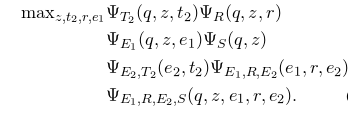
\includegraphics[height=3.5cm]{./1.png}


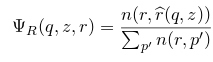
\includegraphics[height=1.5cm]{./2.png}
where
p'
ranges over all phrases that are known to
hint at
r
, and
n
(
r,p
)
denotes the number of sentences where the phrase
p
occurred in the dependency path between the entities participating in relation
r
.

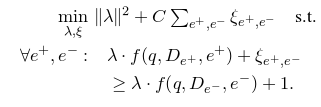
\includegraphics[height=2.8cm]{./3.png}\\
where
e\textsuperscript{+}
and
e\textsuperscript{-}
are positive and negative entities for the query
q
and
f
(
q,D\textsubscript{e}
,e
)
represents the
feature map for the set of snippets
D\textsubscript{e}
belonging
to entity
e
.  The assumption here is that all snip-
pets containing
e\textsuperscript{+}
are “positive” snippets for the
query.
f
consolidates various signals like the number of snippets where
e
occurs near query entity
e\textsubscript{1}
and a relation phrase, or the number of snippets
with high proportion of query IDF, hinting that
e
is a positive entity for the given query.\\

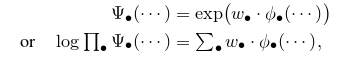
\includegraphics[height=1.8cm]{./4.png}\\

with
w\textsubscript{.}
being a weight vector for a specific potential ., and $ \phi $\textsubscript{.}
being a corresponding feature vector.
During inference, we seek to maximize\\

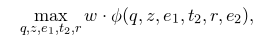
\includegraphics[height=1.5cm]{./5.png}\\

for a fixed
w
, to find the score of each candidate
entity
e
2
.  Here all
w
•
and
φ
•
have been collected
into unified weight and feature vectors
w,φ
. Dur-
ing training of
w
, we are given pairs of correct and
incorrect answer entities
e
+
2
,e
−
2
,  and we wish to
satisfy constraints of the form \\

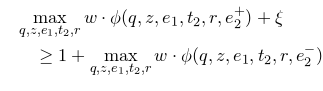
\includegraphics[height=2.3cm]{./6.png}


37
We
propose a structured query mechanism,
entity-relationship
query
, for searching entities in Wikipedia corpus by their
properties and inter-relationships.


